\chapter{Sistema multisensorial }
\label{cap:capitulo4}

%\begin{flushright}
%\begin{minipage}[]{10cm}
%\emph{Quizás algún fragmento de libro inspirador...}\\
%\end{minipage}\\

%Autor, \textit{Título}\\
%\end{flushright}

\vspace{1cm}
Este capítulo consta de la descripción detallada del proceso que se ha llevado a cabo para crear el sistema multisensorial para la monitorización de animales de laboratorio. 

Dos son las partes esenciales para el desarrollo: hardware y software. En la primera sección se presenta el desarrollo hardware y en la sección posterior el desarrollo software que se ha realizado sobre la configuración hardware.

\section{Hardware}
La placa que se ha utilizado para el proyecto es la Raspberry Pi 4B (Figura \ref{fig:rasp}), el último modelo de Raspberry y muy utilizada para el desarrollo de proyectos debido a su bajo coste. Este modelo es el más rápido y potente, ofreciendo de dos a tres veces el rendimiento del procesador de su modelo predecesor. El sistema operativo que utiliza la Raspberry es Raspbian.
\begin{figure} [h!]
  \begin{center}
    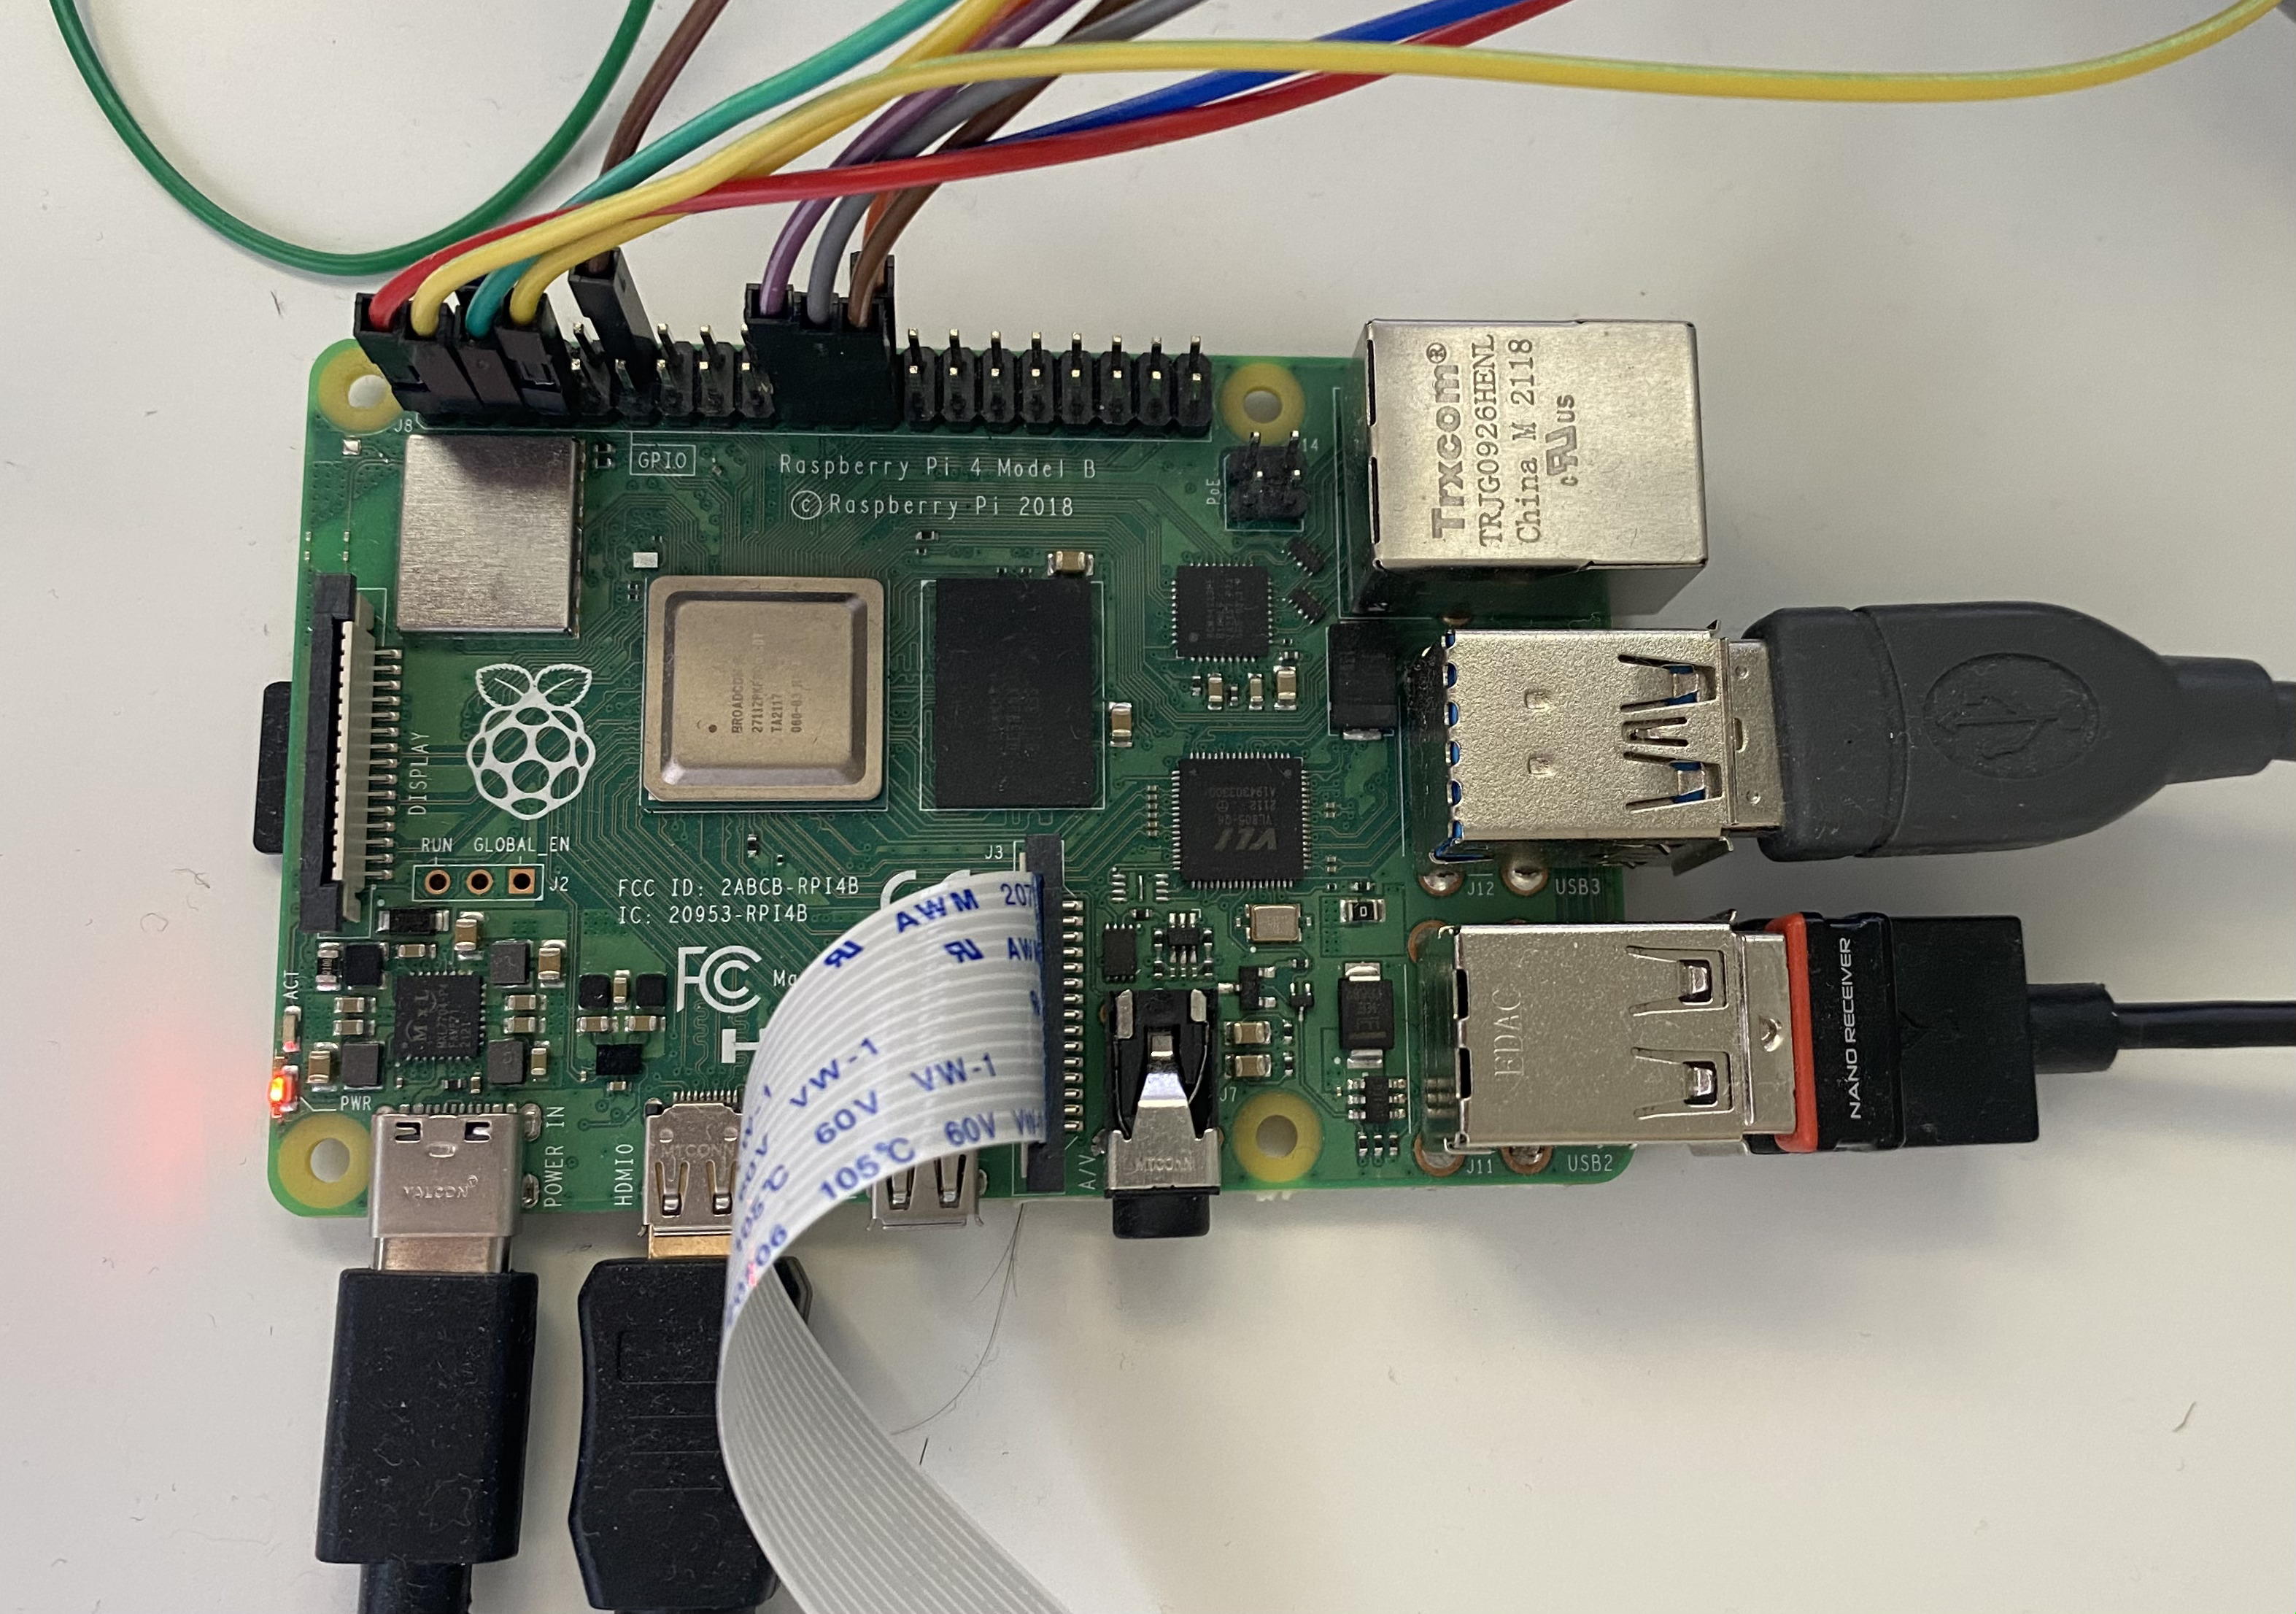
\includegraphics[width=8cm]{figs/raspberry}
  \end{center}
  \caption{Raspberry Pi 4B}
  \label{fig:rasp}
\end{figure}\\

Está dotada de una serie de pines y puertos que permiten su conexión con distintos sensores o actuadores. Para este trabajo se han utilizado los siguientes sensores:
\begin{itemize}
\item{Sensor BME680 (Figura \ref{fig:bme}).} Este sensor es capaz de medir hasta cuatro parámetros: la calidad del aire, la temperatura, la presión y la humedad.
\begin{figure} [h!]
  \begin{center}
    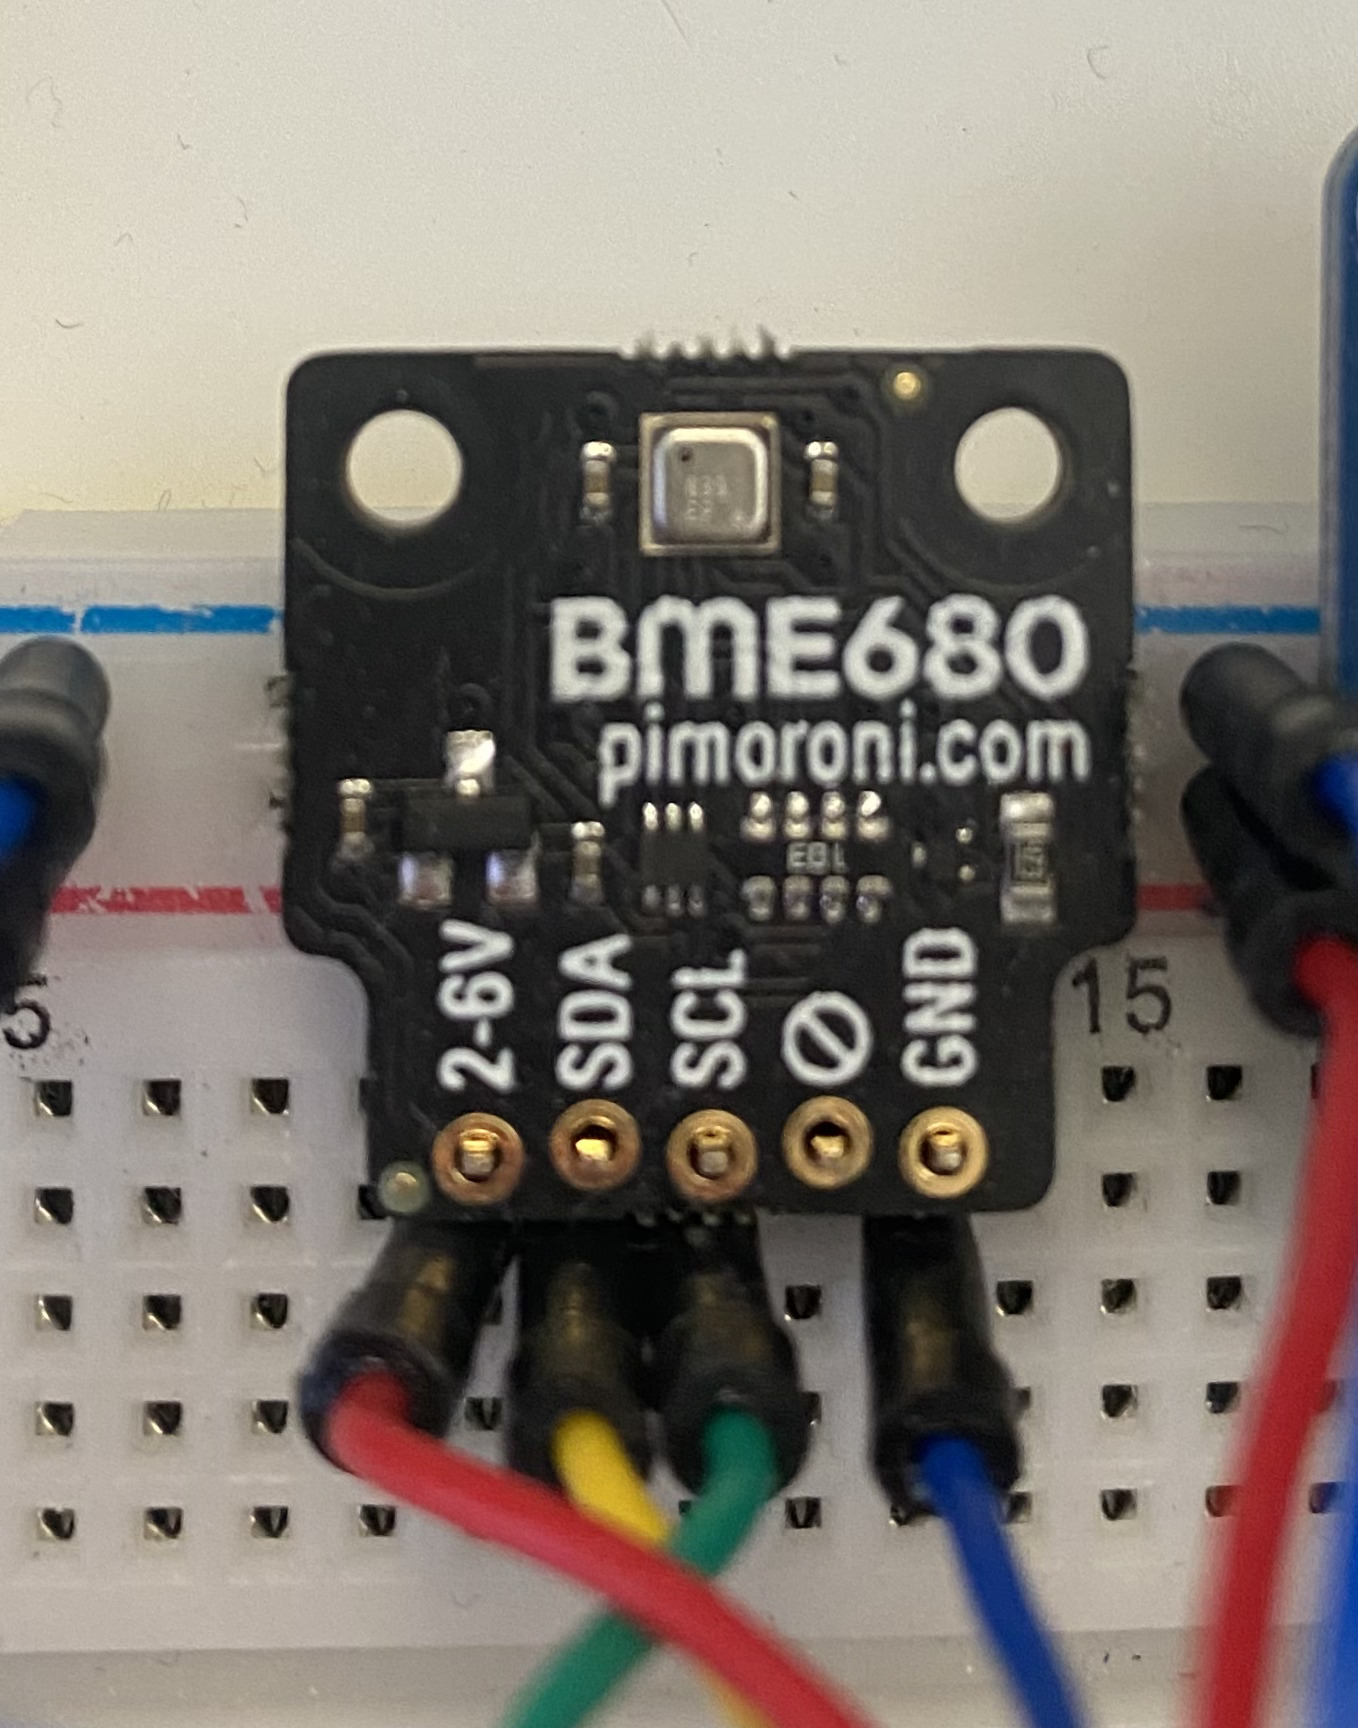
\includegraphics[width=6cm]{figs/bme}
  \end{center}
  \caption{Sensor BME680.}
  \label{fig:bme}
\end{figure}\\

\item{Sensor AMG8833 (Figura \ref{fig:amg}).} Este sensor es una cámara térmica que permite recibir la información del entorno y mostrarla a través de un rango de colores. Los colores más cálidos ---como el rojo--- indican la presencia de mayor temperatura, mientras que los colores fríos ---como el azul--- indican una temperatura inferior.
\begin{figure} [h!]
  \begin{center}
    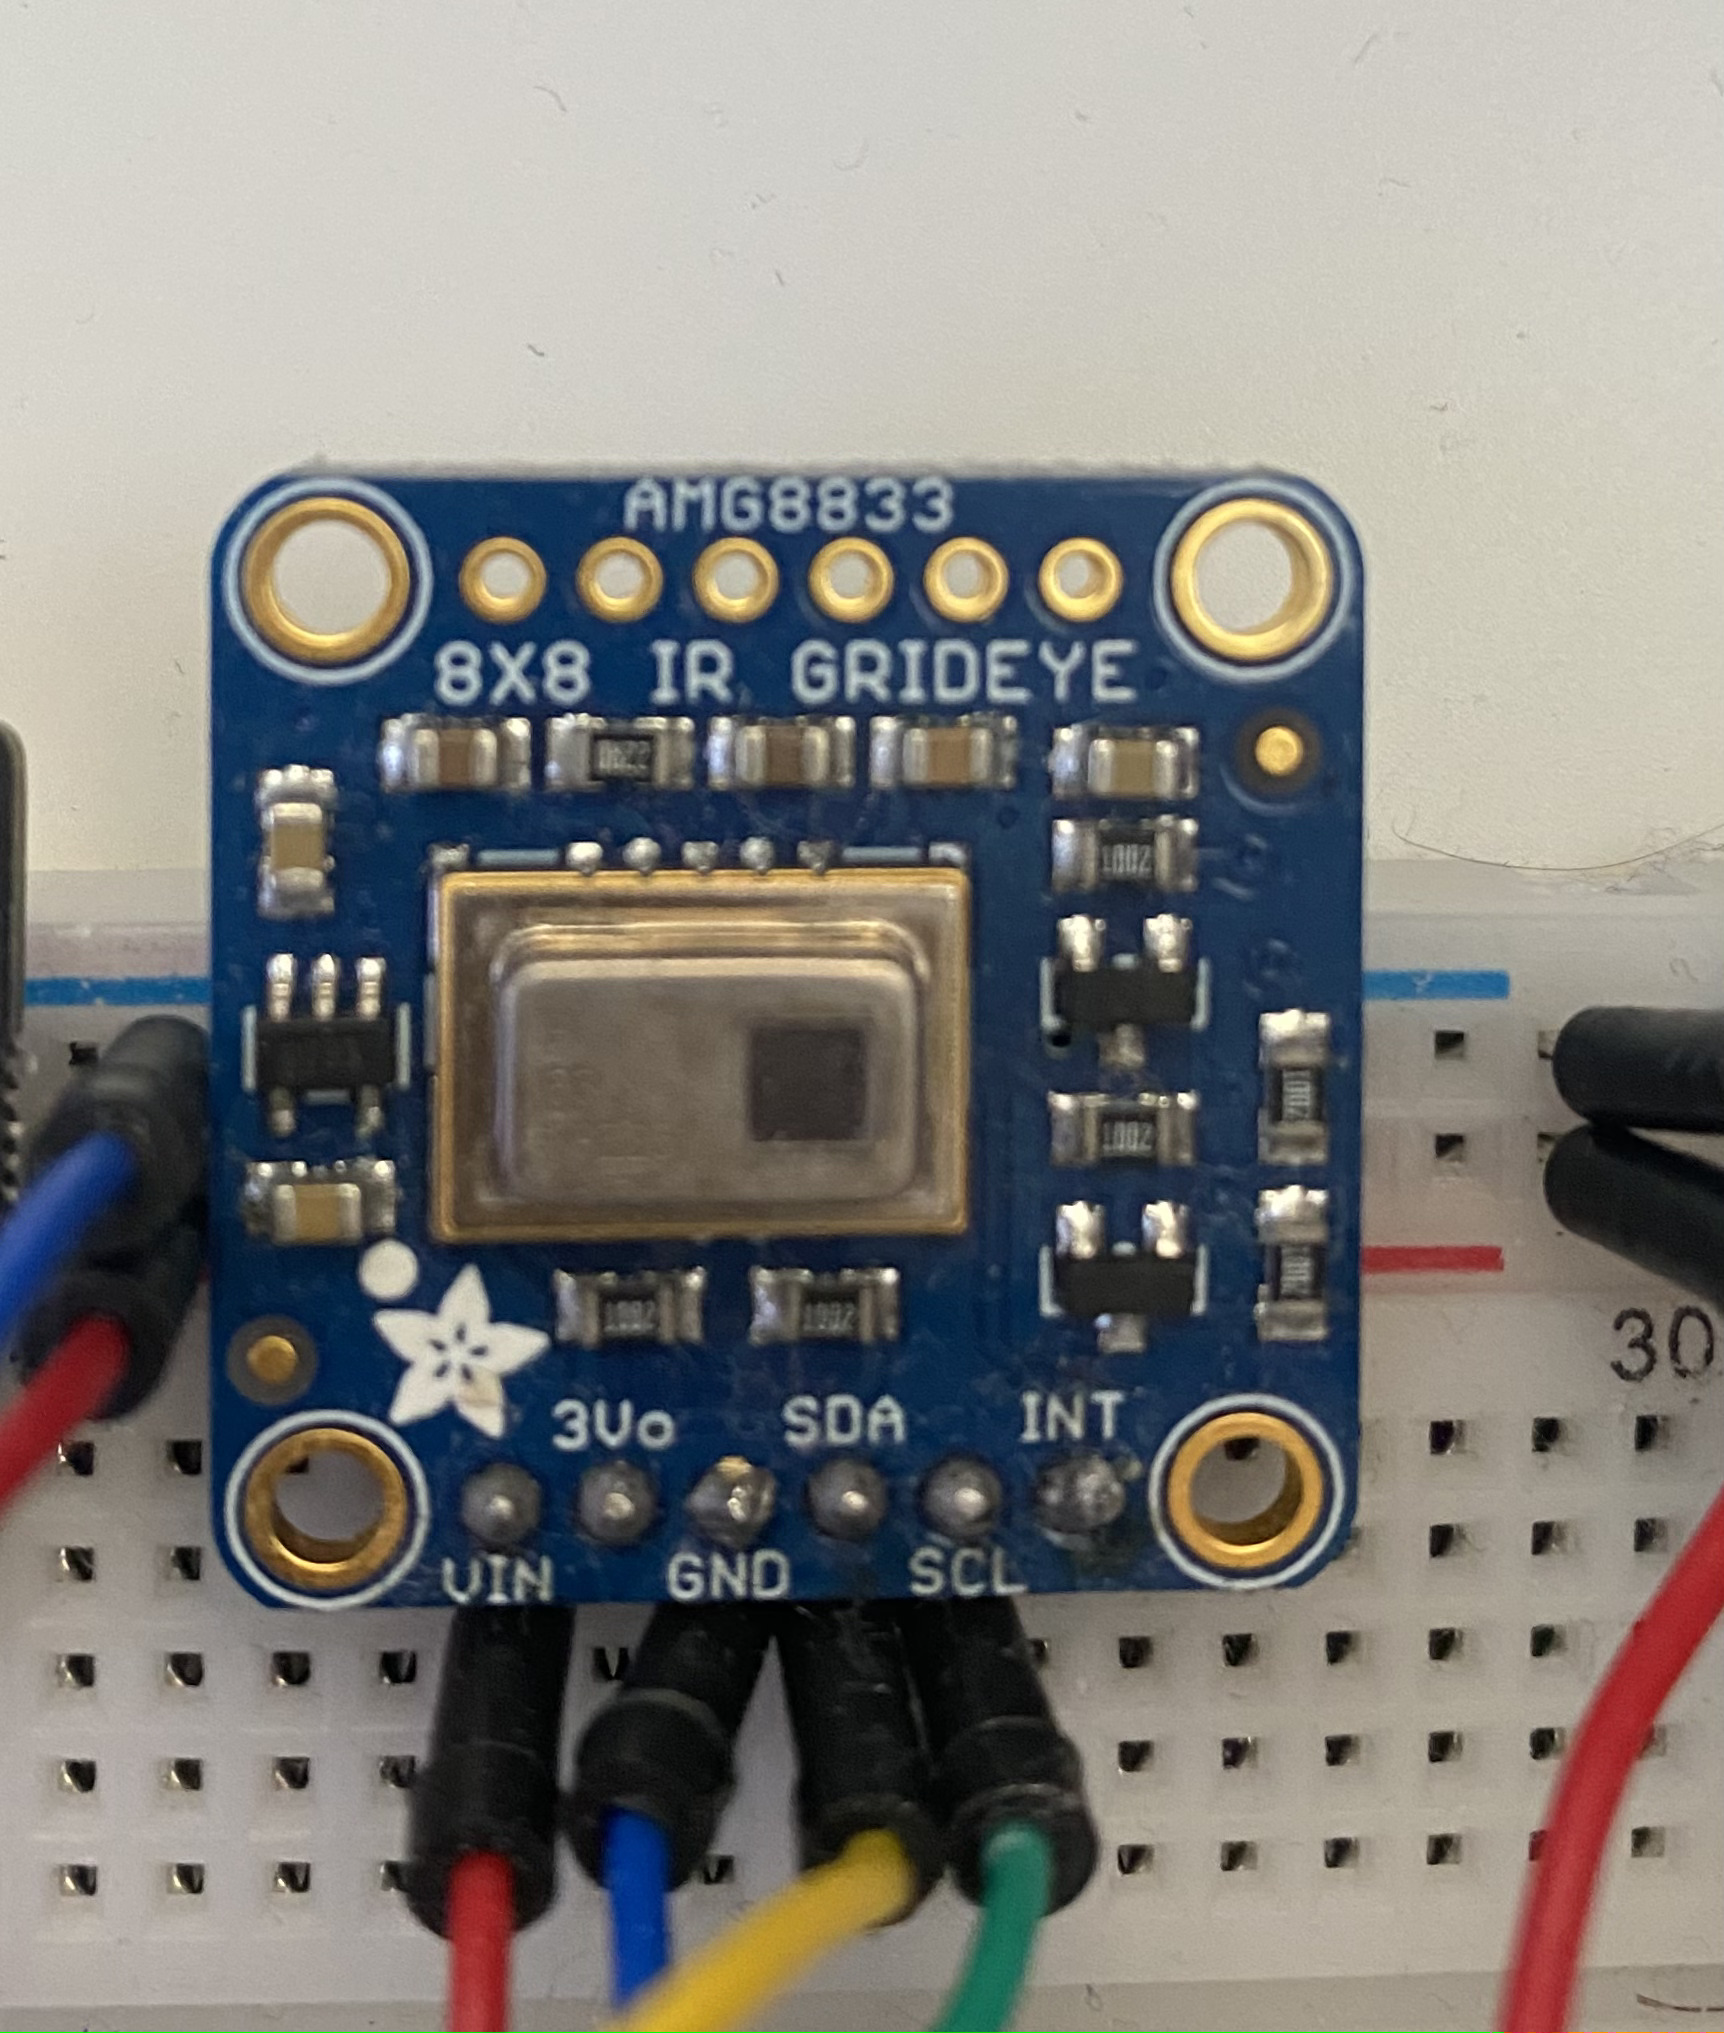
\includegraphics[width=6cm]{figs/amg}
  \end{center}
  \caption{Sensor AMG8833.}
  \label{fig:amg}
\end{figure}\\

\item{Sensor DS18B20 (Figura \ref{fig:ds}).} Este sensor permite medir la temperatura en superficies mojadas, ya que es resistente al agua.
\begin{figure} [h!]
  \begin{center}
    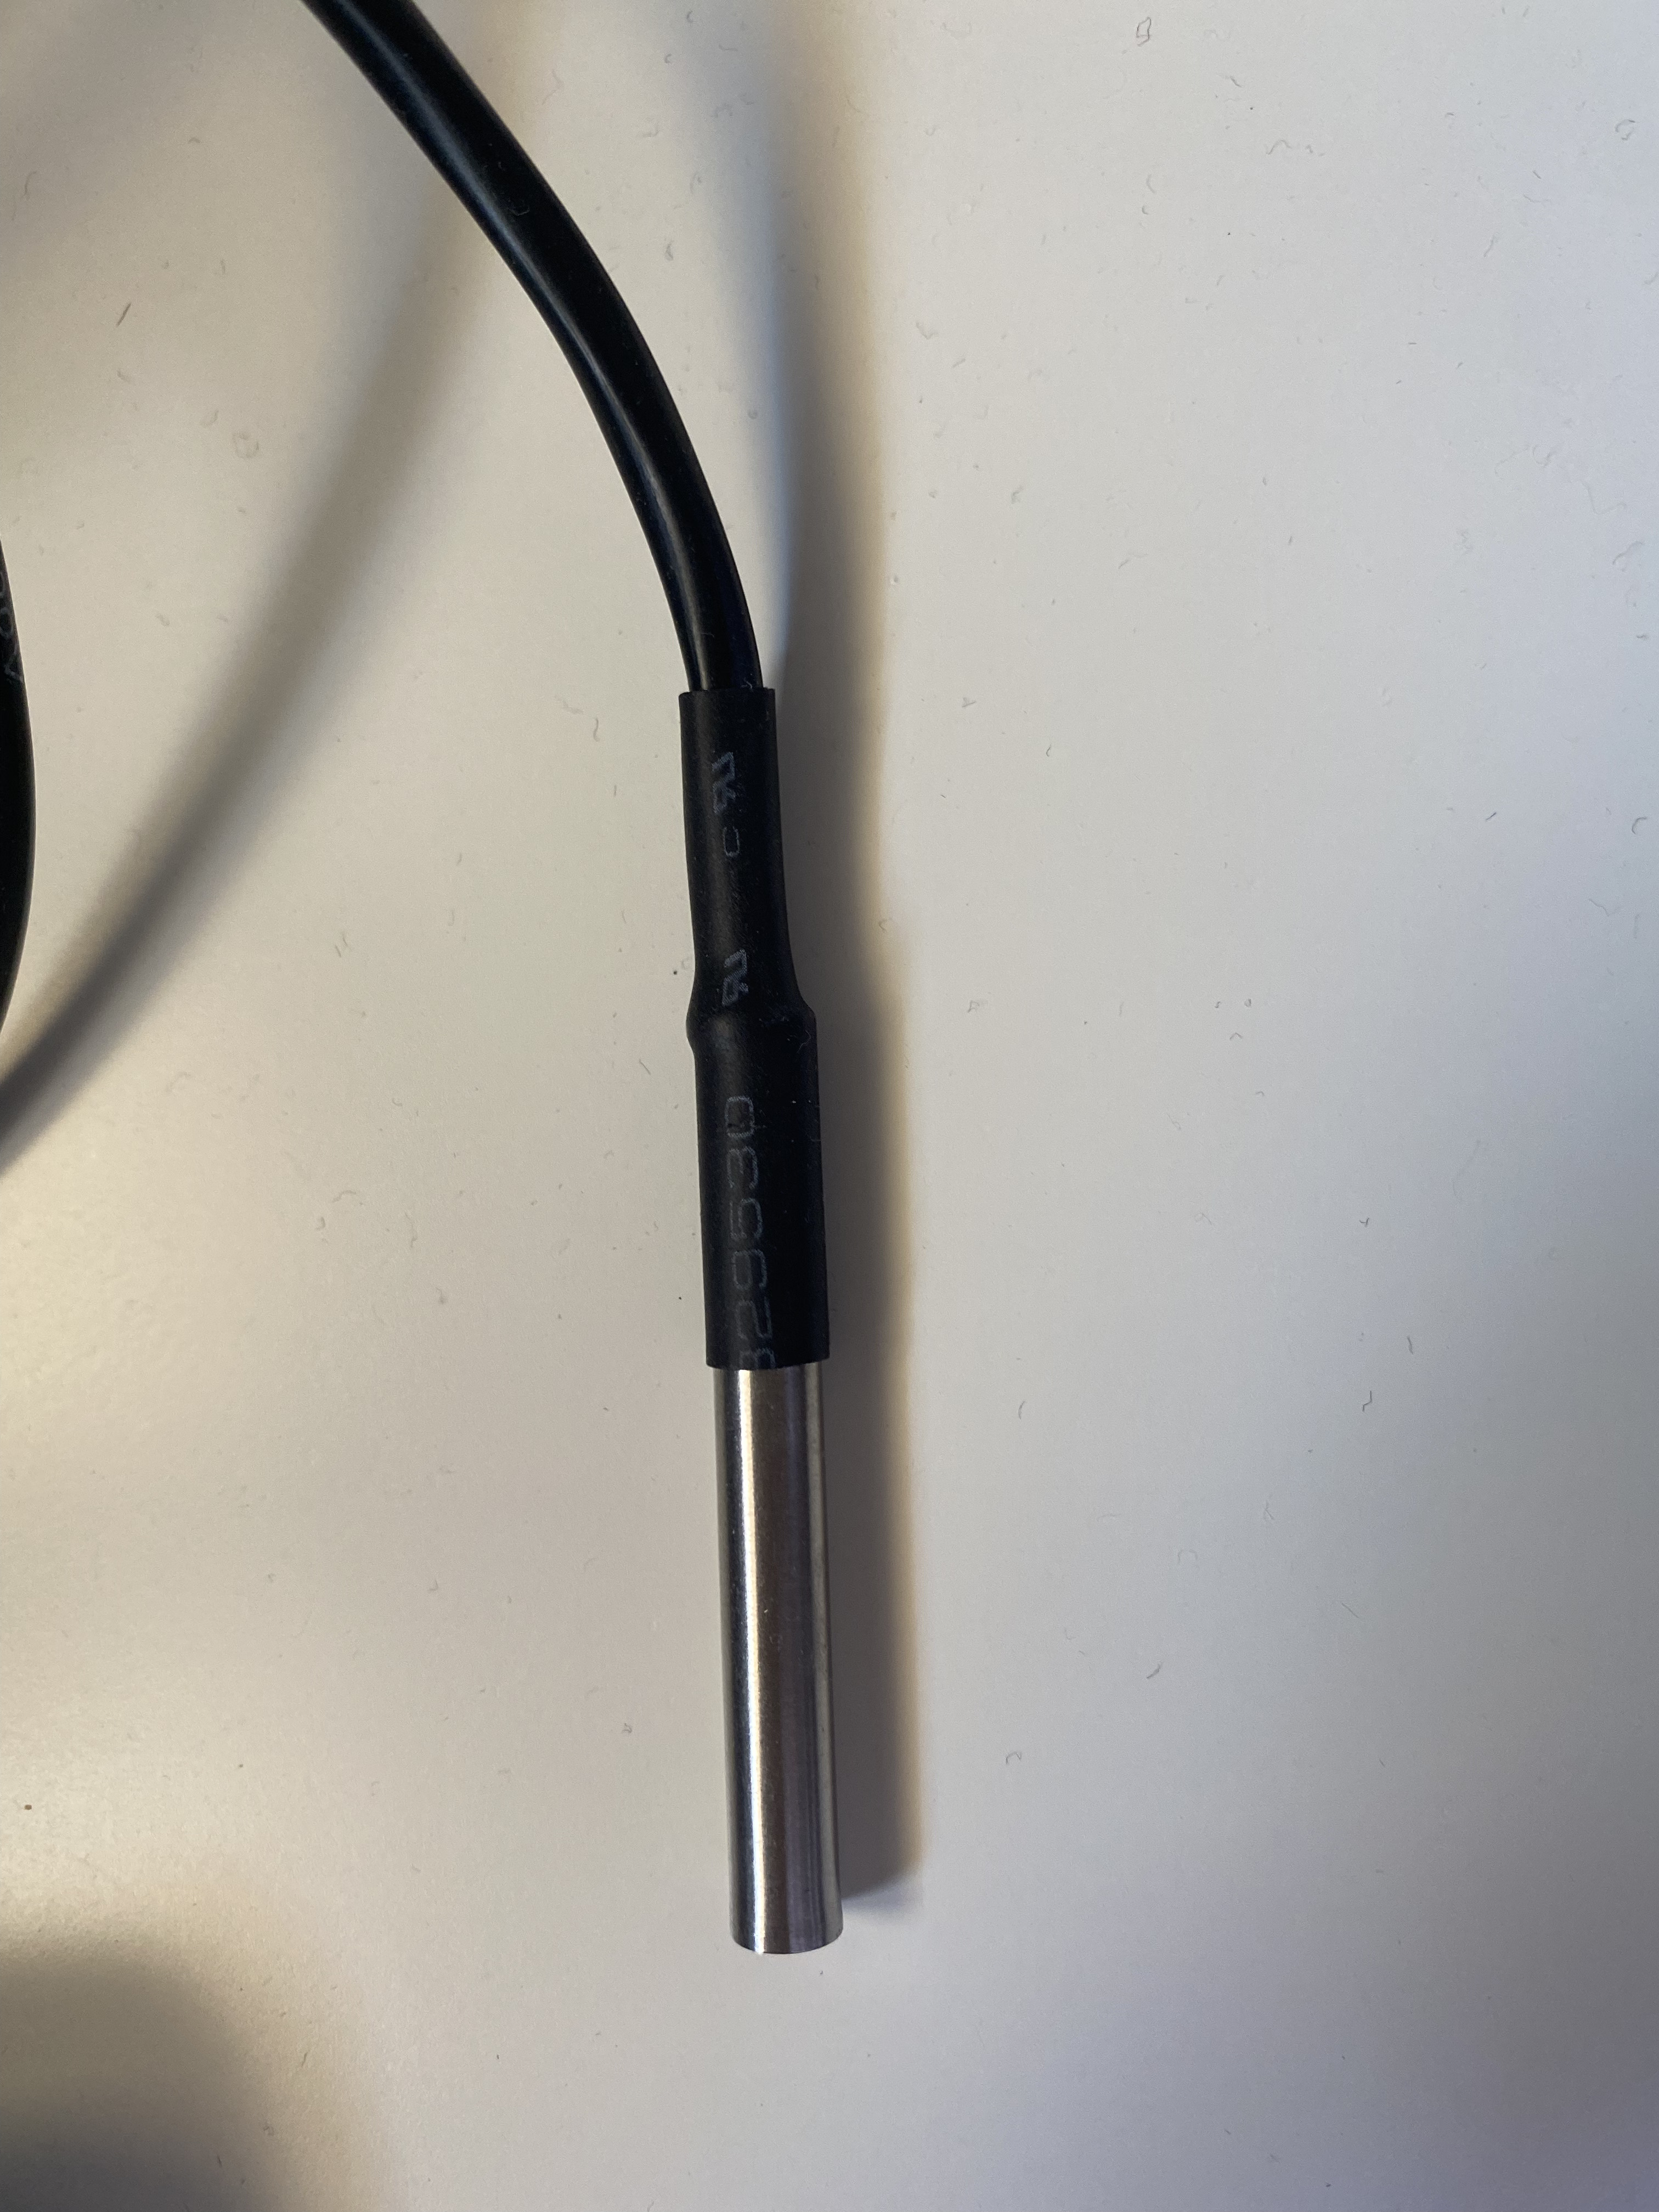
\includegraphics[width=6cm]{figs/ds}
  \end{center}
  \caption{Sensor DS18B20.}
  \label{fig:ds}
\end{figure}\\

\item{MQ-135 (Figura \ref{fig:mq}).} Este sensor permite medir la calidad de distintos gases, entre ellos el de amoníaco.
\begin{figure} [h!]
  \begin{center}
    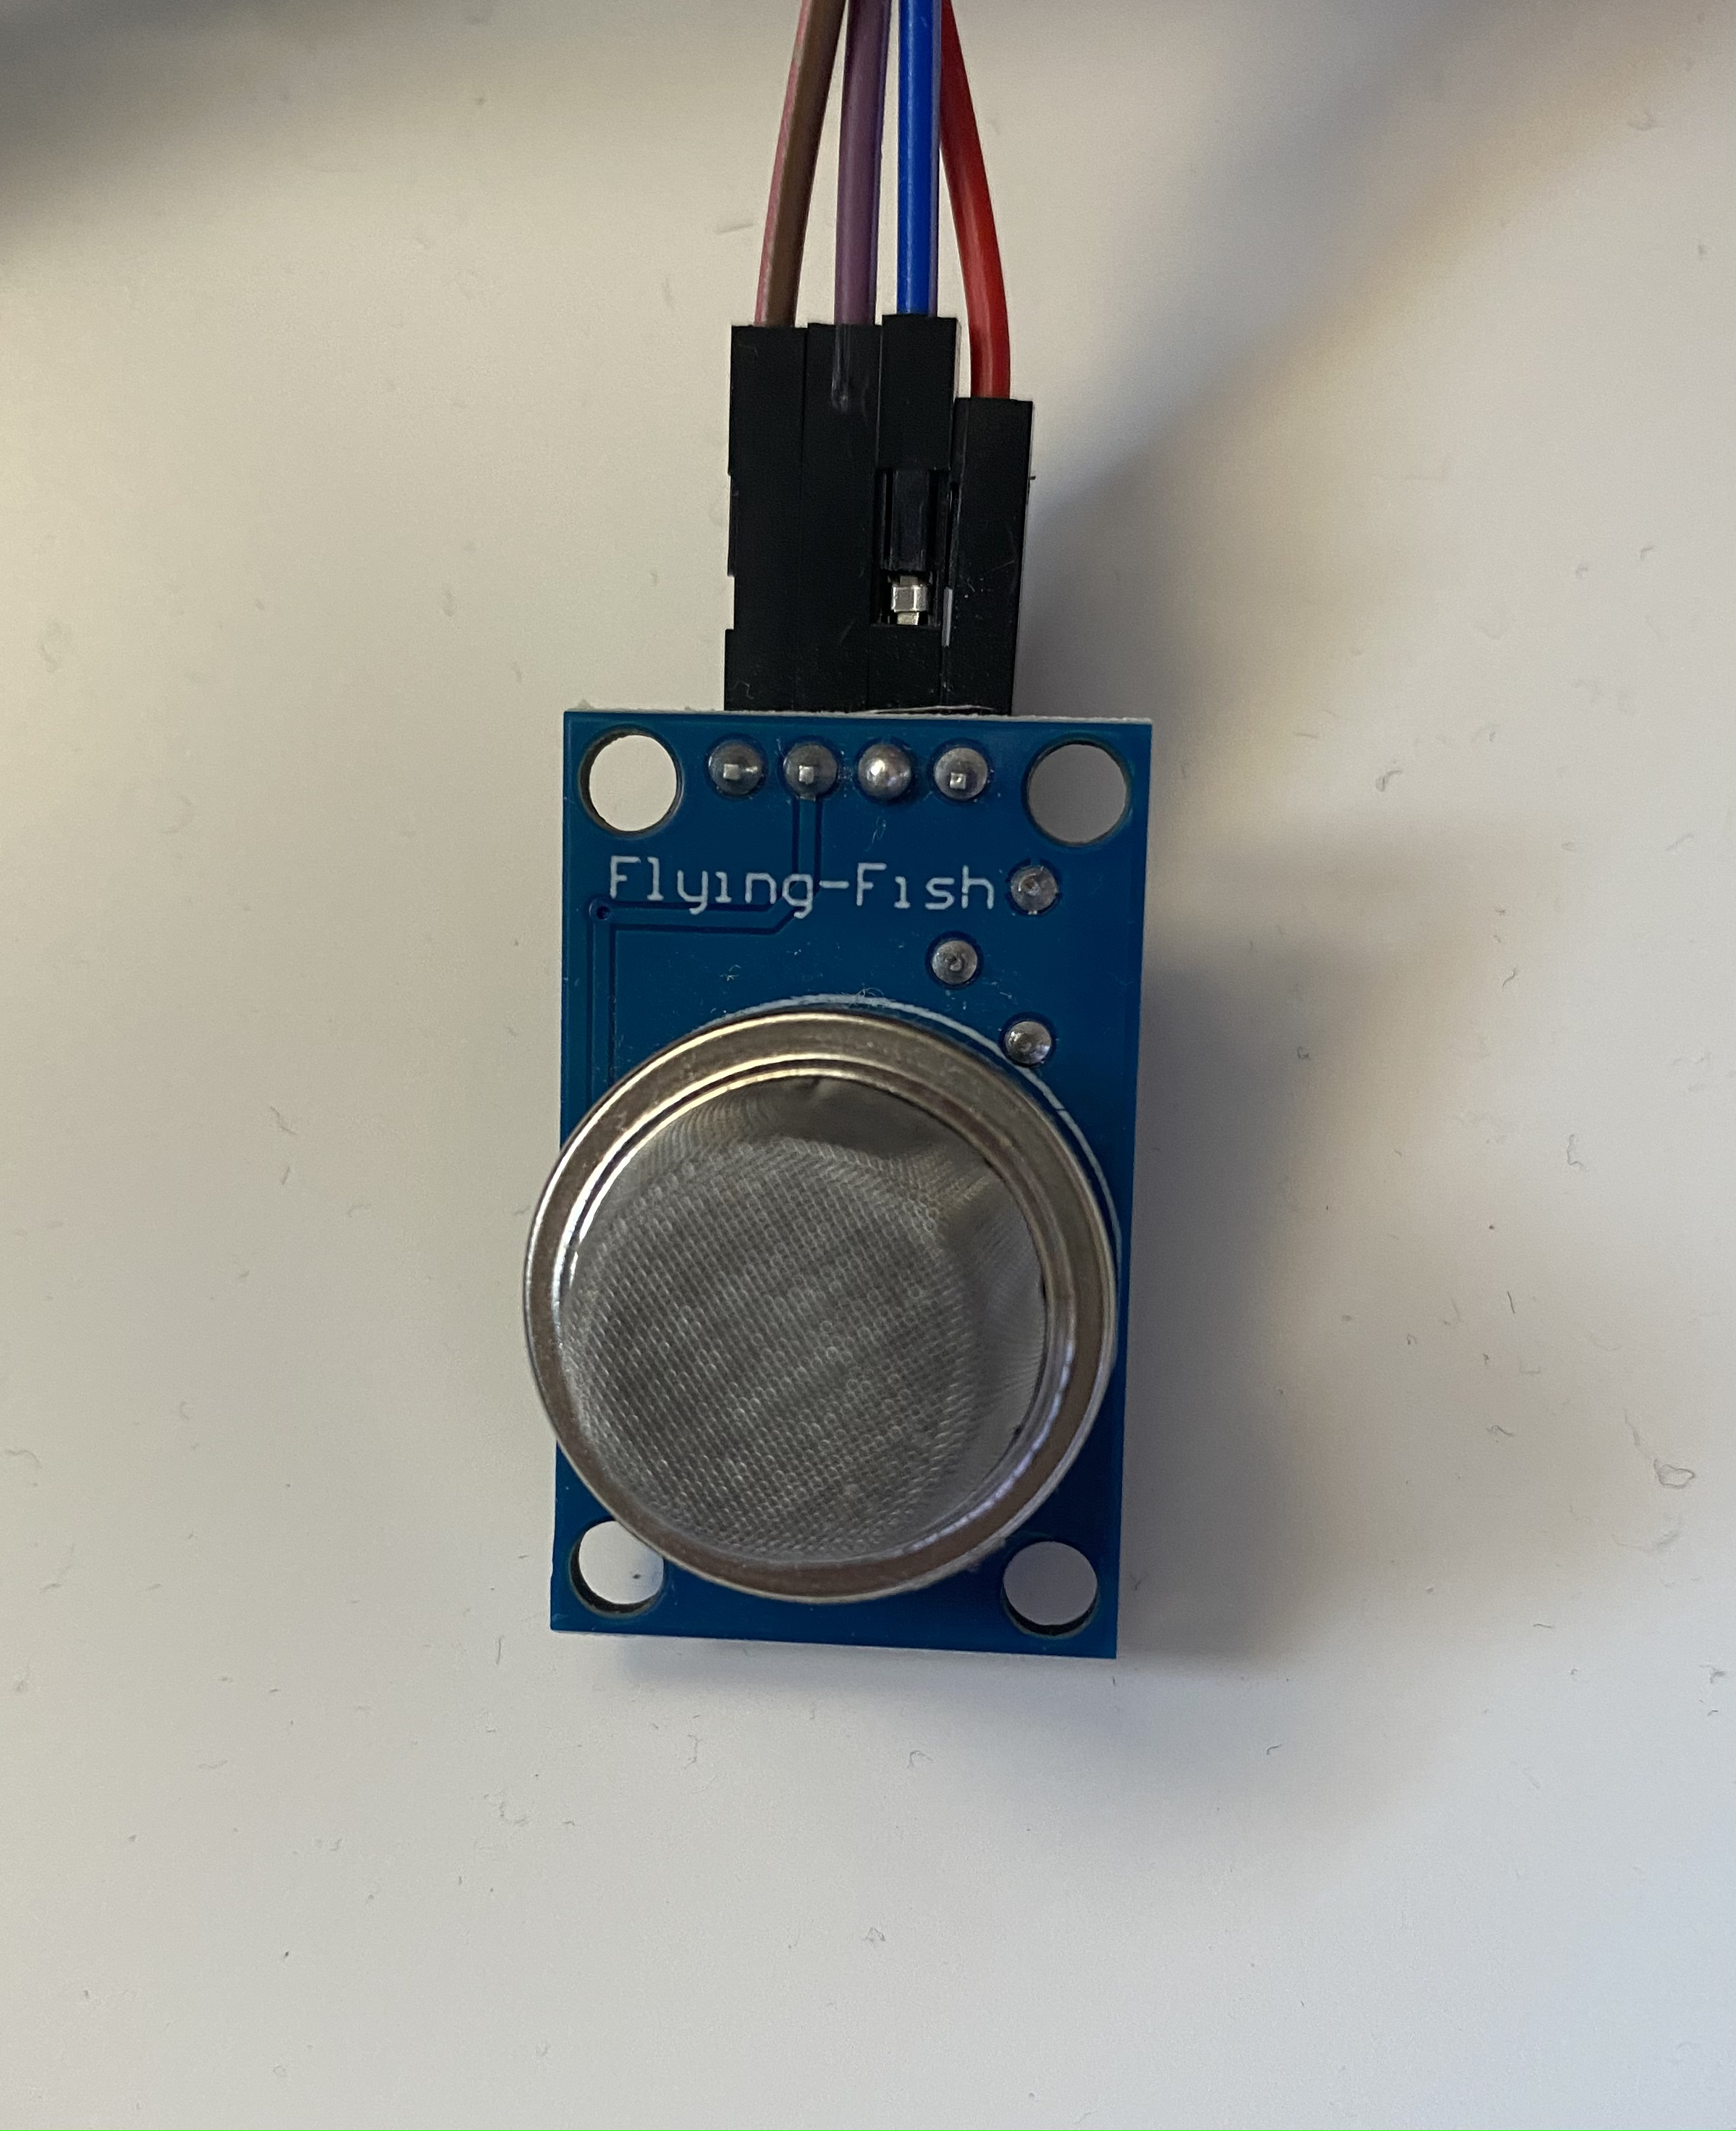
\includegraphics[width=6cm]{figs/mq}
  \end{center}
  \caption{Sensor MQ-135.}
  \label{fig:mq}
\end{figure}\\

\item{Sensor nivel de agua (Figura \ref{fig:nivel}).} Con este sensor se puede medir la presencia de agua, así como la cantidad de agua que hay.
\begin{figure} [h!]
  \begin{center}
    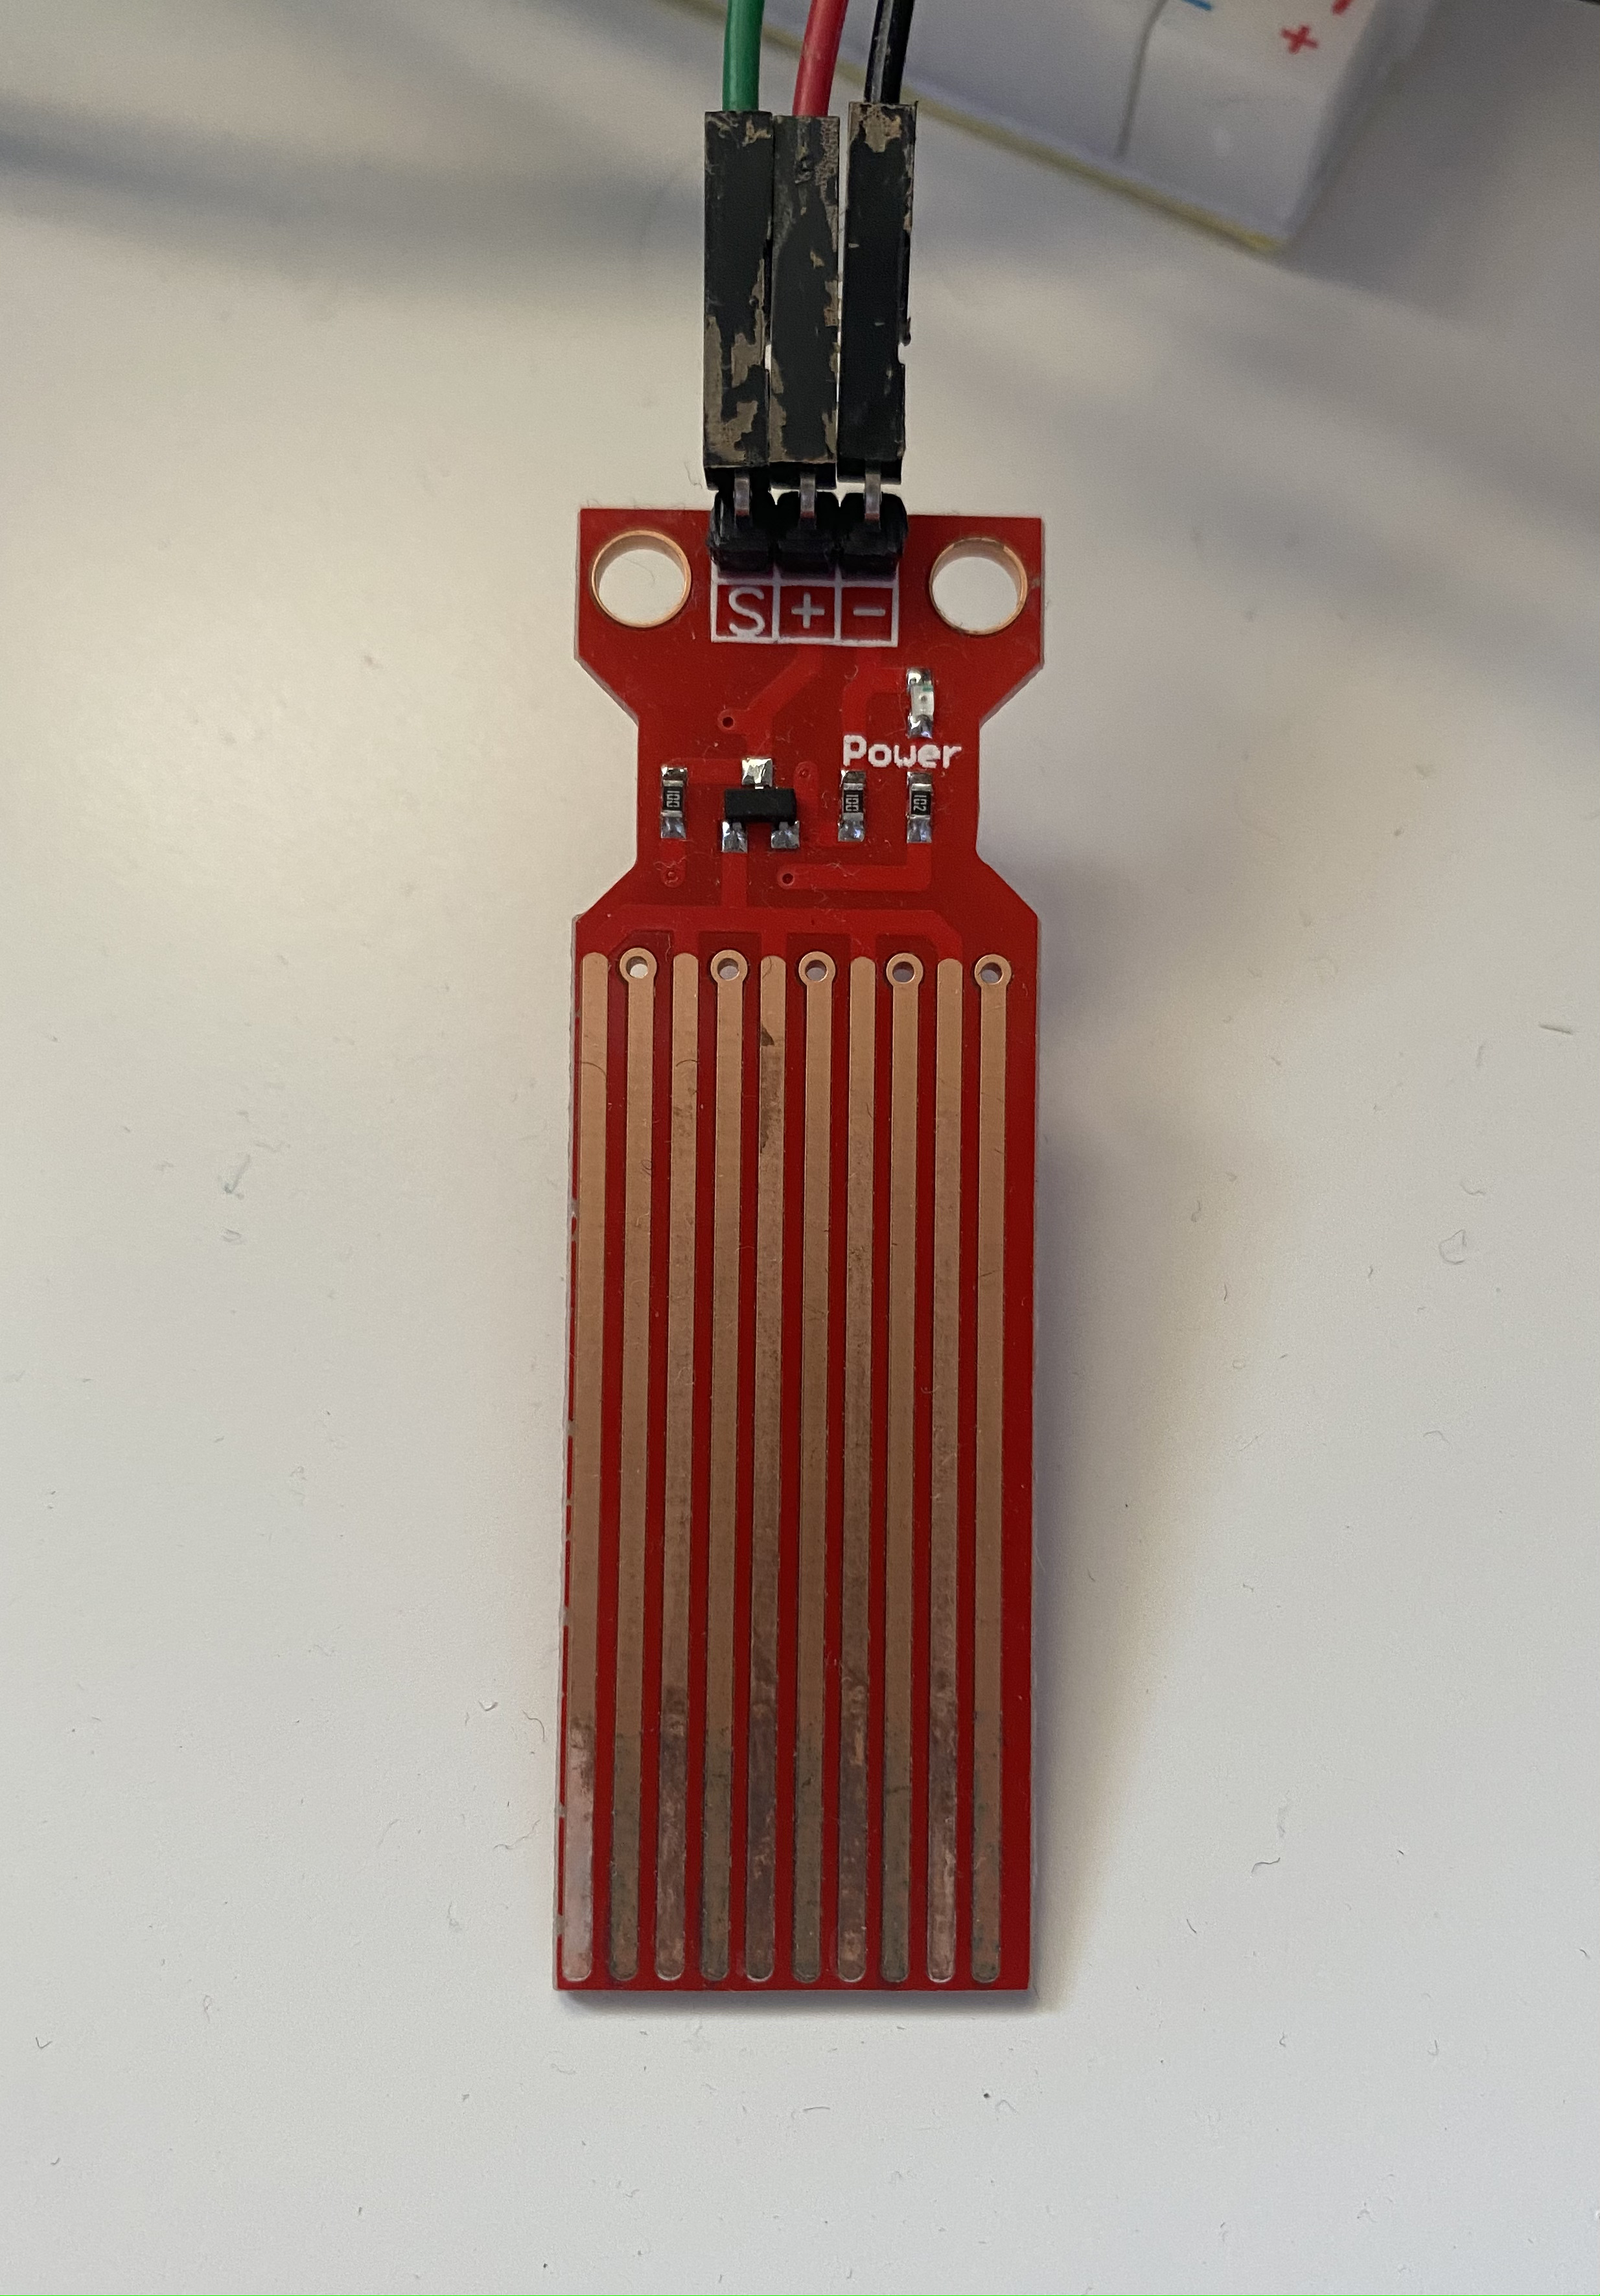
\includegraphics[width=6cm]{figs/nivel}
  \end{center}
  \caption{Sensor de nivel de agua.}
  \label{fig:nivel}
\end{figure}\\

%\item{Sensor AM2315 (Figura \ref{fig:am}).} Este sensor permite medir tanto la temperatura como la humedad.
%\begin{figure} [h!]
%  \begin{center}
%    \includegraphics[width=6cm]{figs/am}
%  \end{center}
%  \caption{Sensor AM2315.}
%  \label{fig:ds}
%\end{figure}\\

\item{Seek thermal (Figura \ref{fig:seek}).} Este sensor es una cámara térmica. Permite obtener imágenes representando las temperaturas con colores de la misma forma que el sensor \ref{fig:amg}, pero con mucha más calidad y precisión.\begin{figure} [h!]
  \begin{center}
    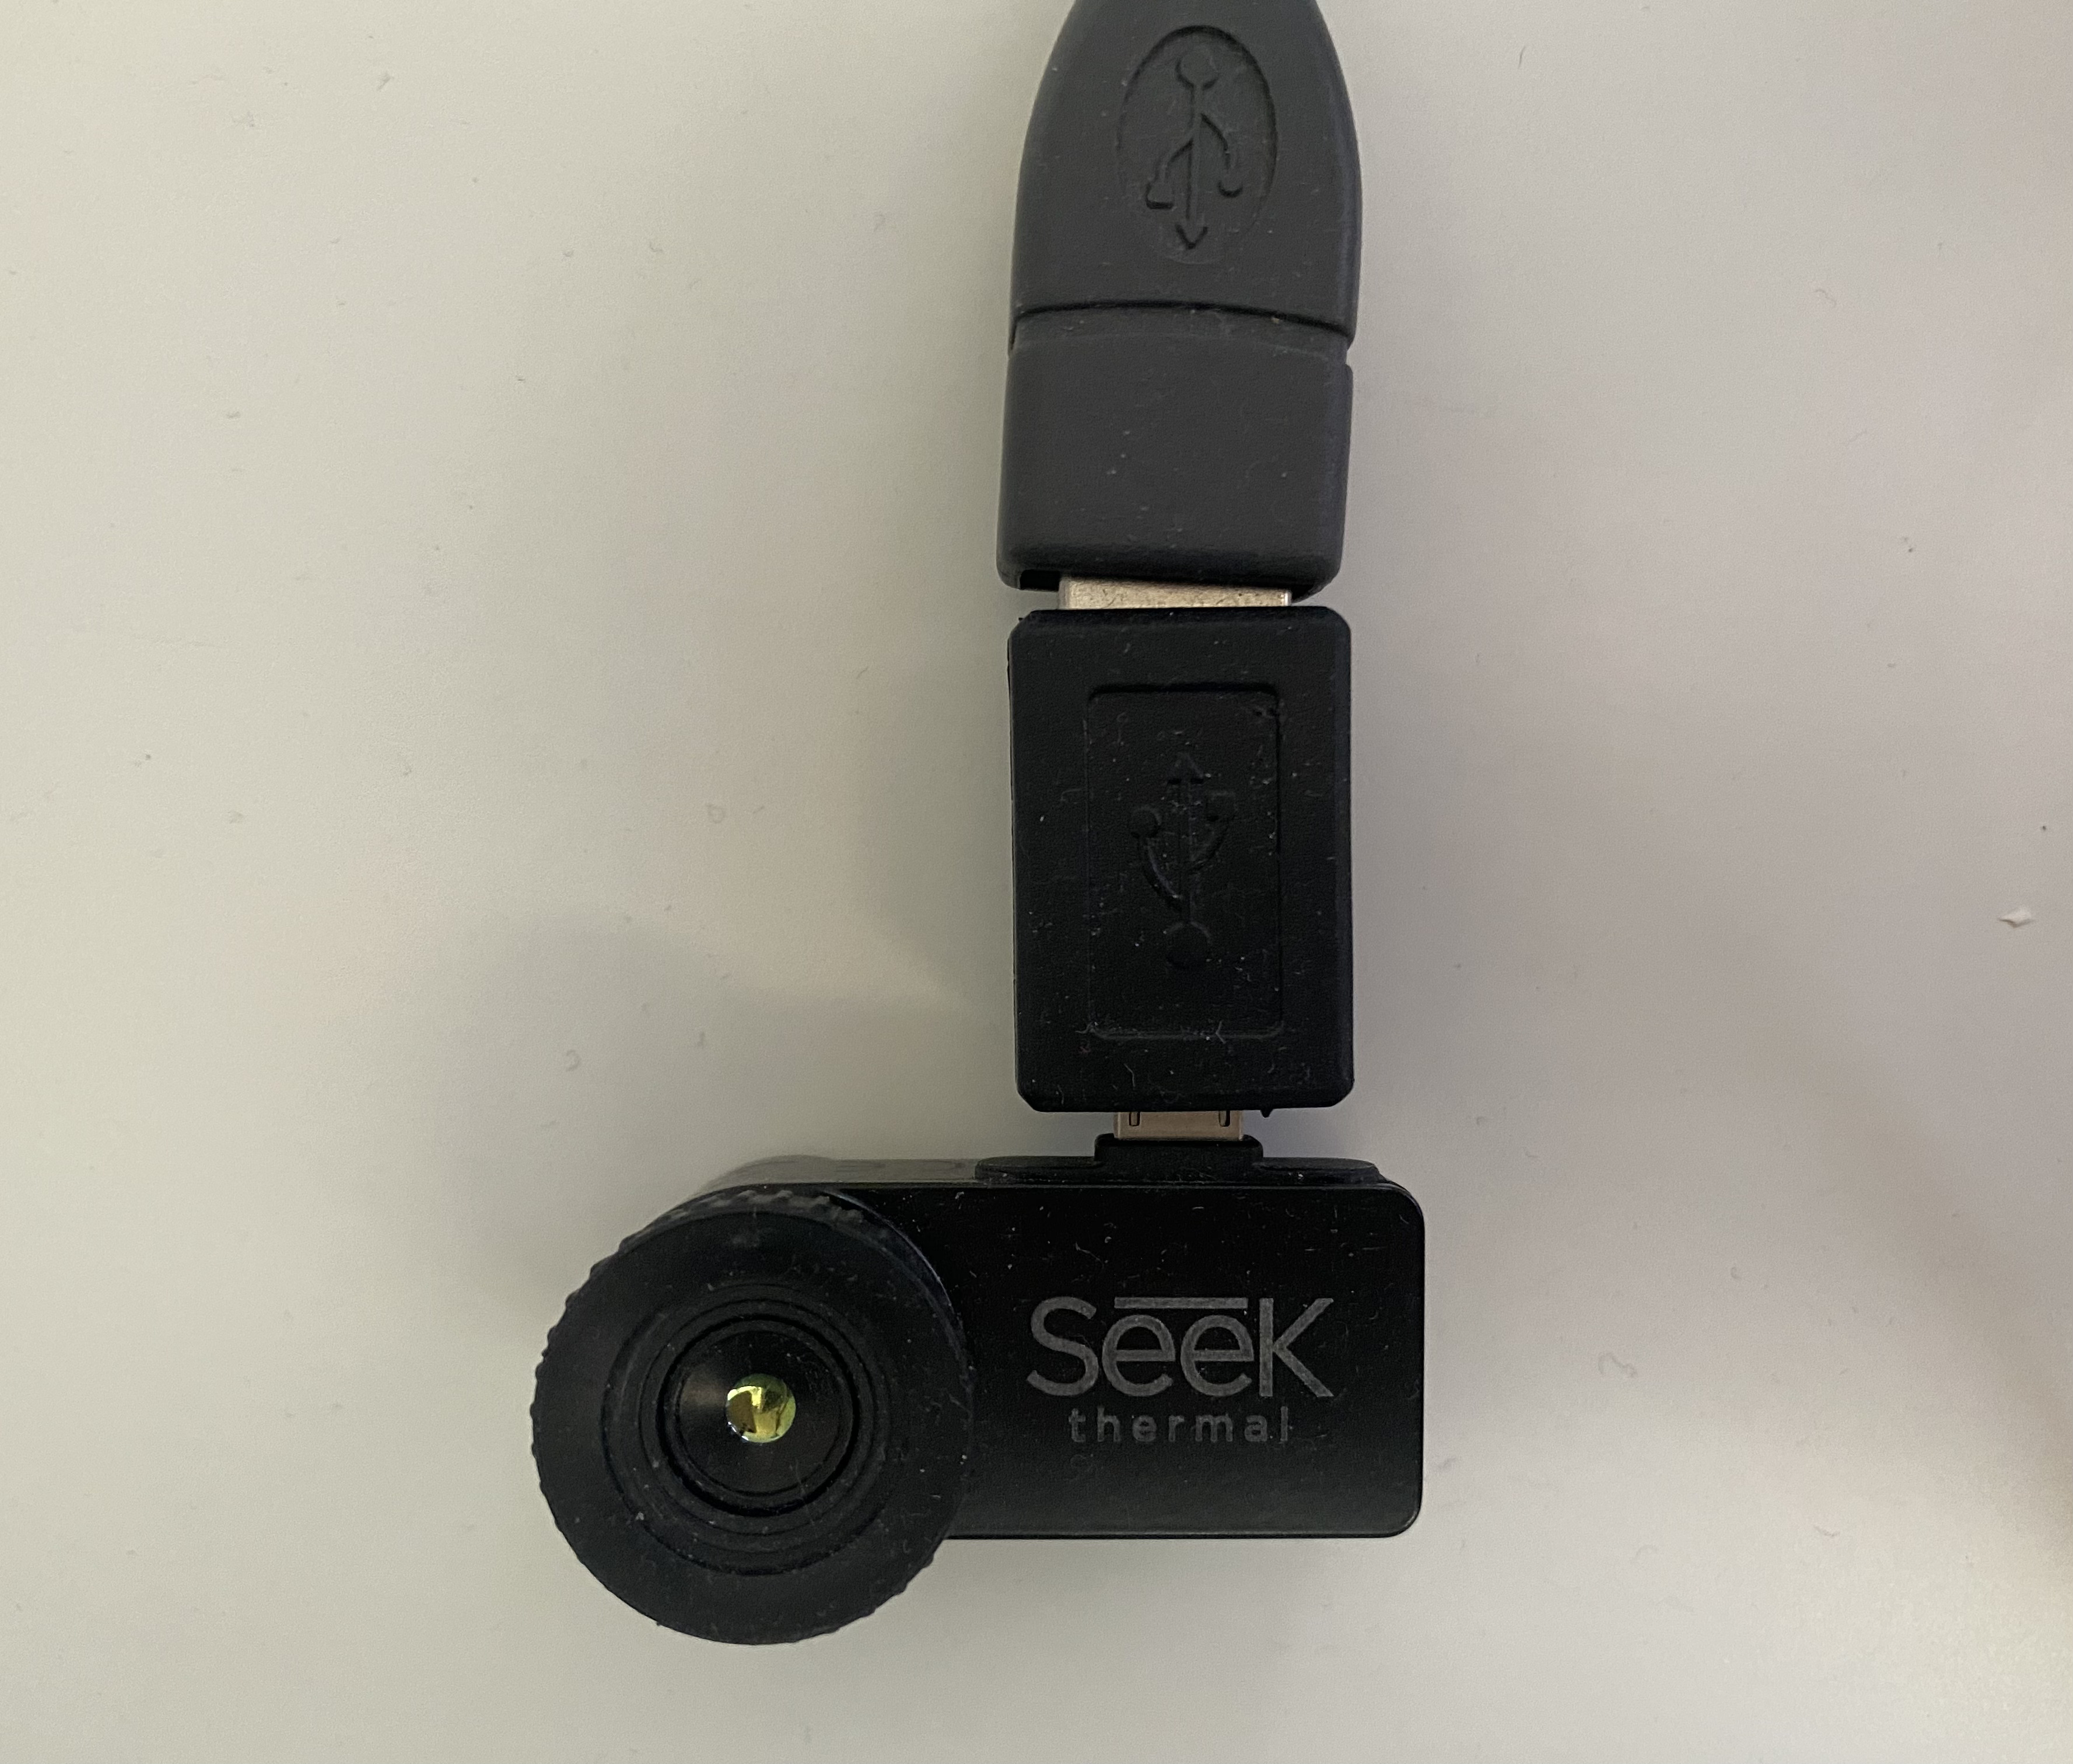
\includegraphics[width=6cm]{figs/seek}
  \end{center}
  \caption{Cámara térmica.}
  \label{fig:seek}
\end{figure}\\

\item{PiCamera (Figura \ref{fig:picam}).} Este sensor es una de las cámaras oficiales de Raspberry, que permite obtener imágenes del entorno y mostrarlas en pantalla.
\begin{figure} [h!]
  \begin{center}
    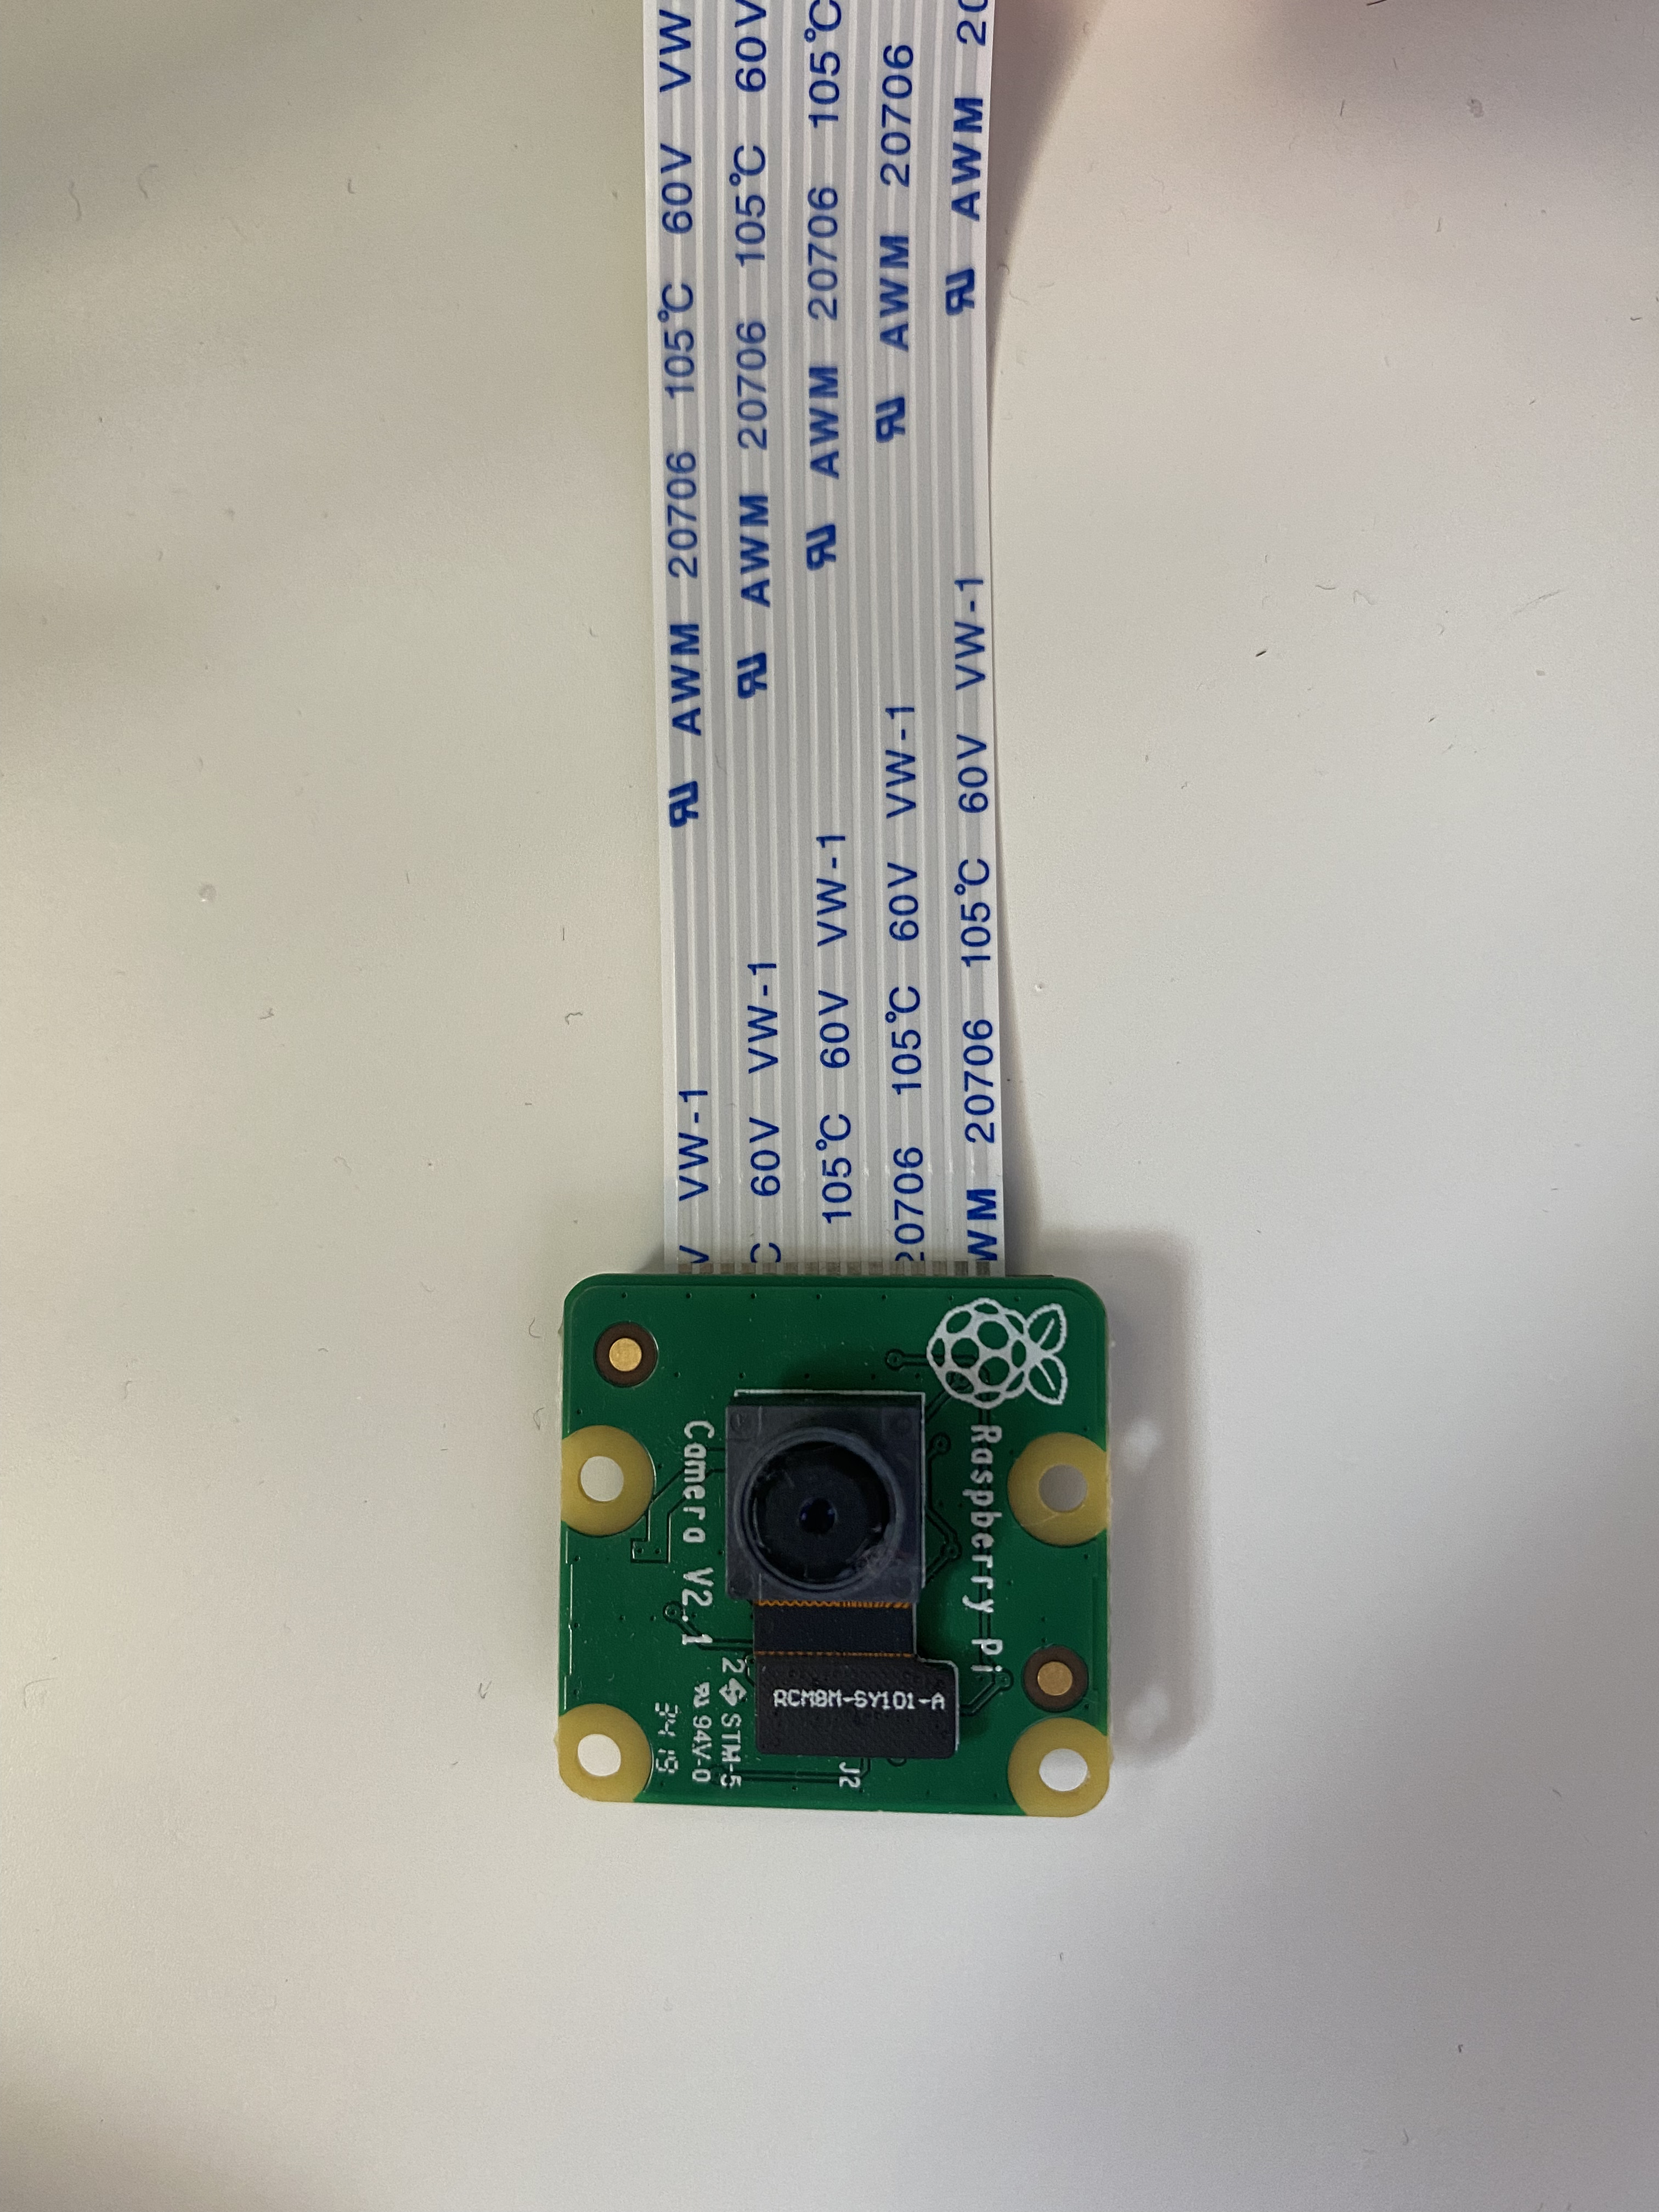
\includegraphics[width=6cm]{figs/picam}
  \end{center}
  \caption{Cámara de Raspberry.}
  \label{fig:picam}
\end{figure}\\
\end{itemize}

Además de los sensores, se han utilizado otros componentes como son resistencias, un led o un conversor analógico a digital para el correcto funcionamiento de los sensores y proporcionar mayor comprensión al funcionamiento del sistema.

En la figura \ref{fig:esquema} se puede ver un esquema de la conexión de los sensores mencionados en la Raspberry.
\begin{figure} [h!]
  \begin{center}
    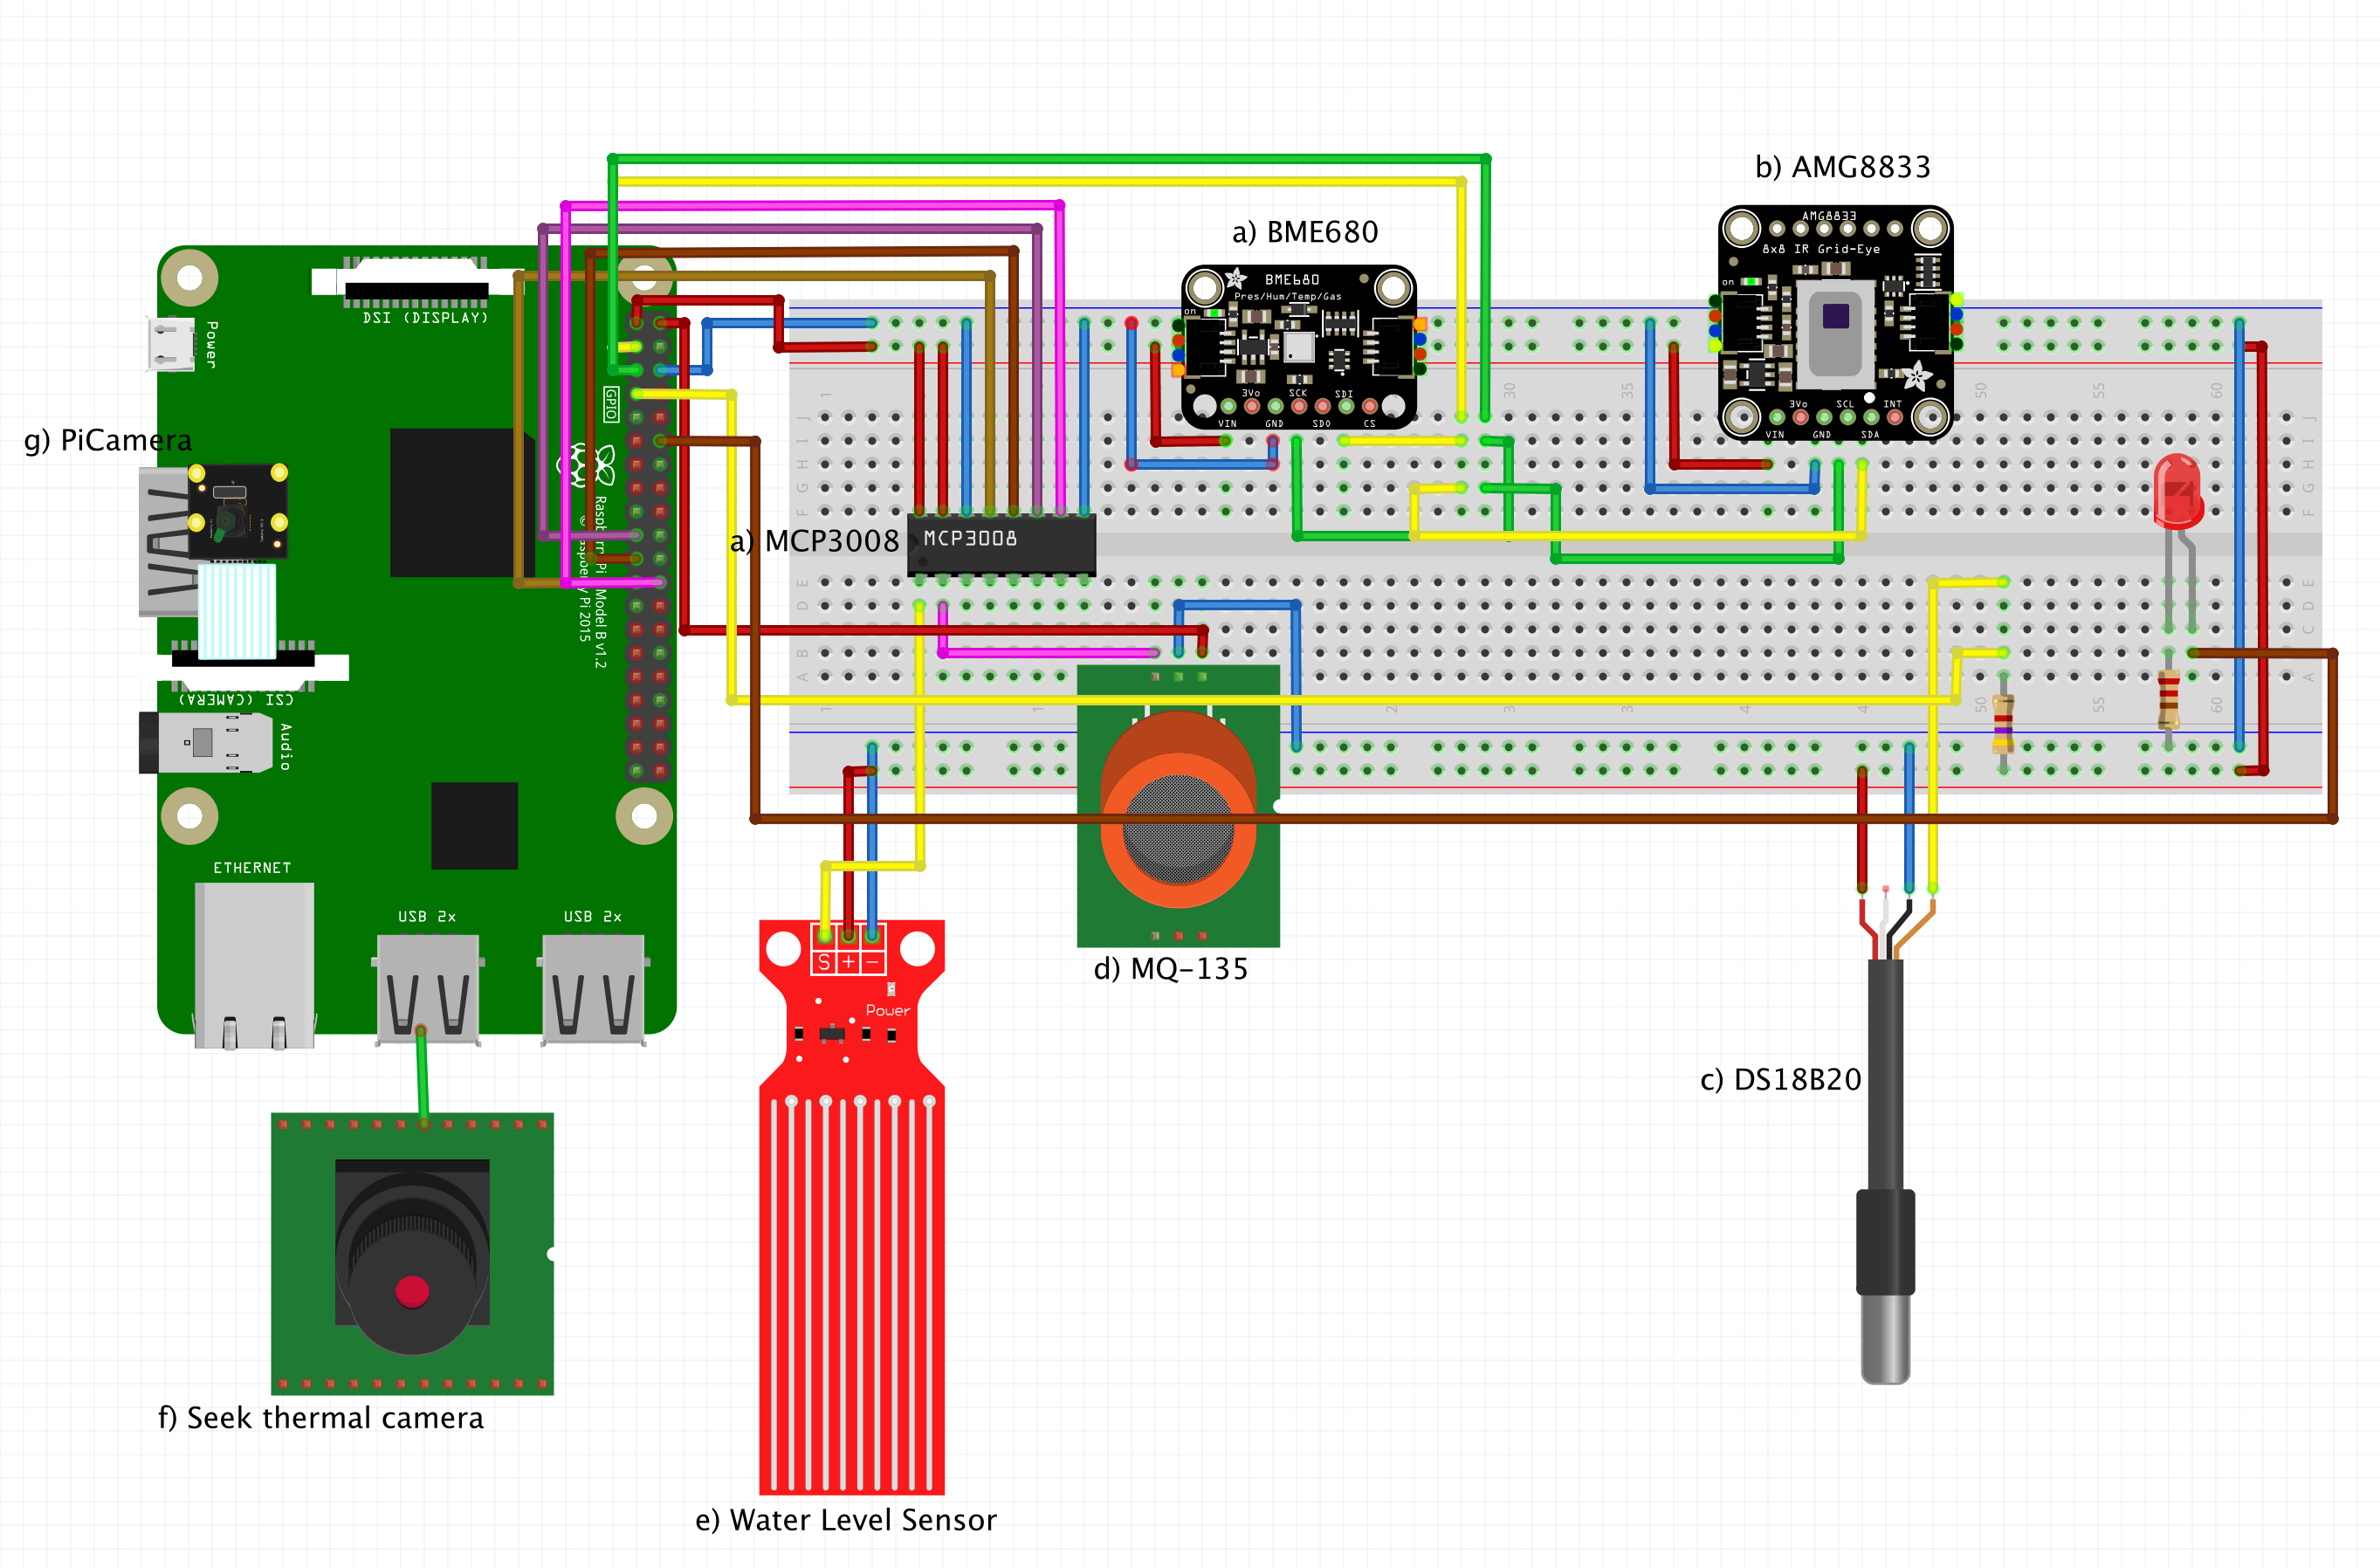
\includegraphics[width=14cm]{figs/esquema}
  \end{center}
  \caption{Esquema de conexiones.}
  \label{fig:esquema}
\end{figure}\\












Puede resultar interesante, para clarificar la descripción, mostrar fragmentos de código (o \textit{snippets}) ilustrativos. En el Código \ref{cod:codejemplo} vemos un ejemplo escrito en \texttt{C++}.

\begin{code}[h]
\begin{lstlisting}[language=C++]
void Memory::hypothesizeParallelograms () {
  for(it1 = this->controller->segmentMemory.begin(); it1++) {
    squareFound = false; it2 = it1; it2++;
    while ((it2 != this->controller->segmentMemory.end()) && (!squareFound)) {
      if (geometry::haveACommonVertex((*it1),(*it2),&square)) {
        dist1 = geometry::distanceBetweenPoints3D ((*it1).start, (*it1).end);
        dist2 = geometry::distanceBetweenPoints3D ((*it2).start, (*it2).end);
      }
    // [...]
\end{lstlisting}
\caption[Función para buscar elementos 3D en la imagen]{Función para buscar elementos 3D en la imagen}
\label{cod:codejemplo}
\end{code}

En el Código \ref{cod:codejemplo2} vemos un ejemplo escrito en \texttt{Python}.

\begin{code}[h]
\begin{lstlisting}[language=Python]
def mostrarValores():
    print (w1.get(), w2.get())

master = Tk()
w1 = Scale(master, from_=0, to=42)
w1.pack()
w2 = Scale(master, from_=0, to=200, orient=HORIZONTAL)
w2.pack()
Button(master, text='Show', command=mostrarValores).pack()

mainloop()
\end{lstlisting}
\caption[Cómo usar un Slider]{Cómo usar un Slider}
\label{cod:codejemplo2}
\end{code}

\section{Verbatim}

Para mencionar identificadores usados en el código ---como nombres de funciones o variables--- en el texto, usa el entorno literal o verbatim \verb|hypothesizeParallelograms()|. También se puede usar este entorno para varias líneas, como se ve a continuación:

\begin{verbatim}
void Memory::hypothesizeParallelograms () {
  // add your code here
}
\end{verbatim}

\section{Ecuaciones}

Si necesitas insertar alguna ecuación, puedes hacerlo. Al igual que las figuras, no te olvides de referenciarlas. A continuación se exponen algunas ecuaciones de ejemplo: Ecuación \ref{ec:ec1} y Ecuación \ref{ec:ec2}.

\begin{myequation}[h]
\begin{equation}
H = 1 - \frac{\sum_{i=0}^{N}\frac{(\frac{d_{j_s} + d_{j_e}}{2})}{N}}{M}
\nonumber
\label{ec:ec1}
\end{equation}
\caption[Ejemplo de ecuación con fracciones]{Ejemplo de ecuación con fracciones}
\end{myequation} 

\begin{myequation}[h]
\begin{equation}
v(entrada)= \left\{
	\begin{array}{lcc}
		0 & \mbox{if} & \epsilon_t < 0.1\\
		K_p\cdot{(T_{t}-T)} & \mbox{if}& 0.1 \leq \epsilon_t < M_t\\
		K_p \cdot M_t & \mbox{if}& M_t < \epsilon_t
	\end{array}
\right.
\label{ec:ec2}
\end{equation}
\caption[Ejemplo de ecuación con array y letras y símbolos especiales]{Ejemplo de ecuación con array y letras y símbolos especiales}
\end{myequation}

\section{Tablas o cuadros}

Si necesitas insertar una tabla, hazlo dígnamente usando las propias tablas de \LaTeX, no usando pantallazos e insertándolas como figuras... En el Cuadro \ref{cuadro:ejemplo} vemos un ejemplo.

\begin{table}[H]
\begin{center}
\begin{tabular}{|c|c|}
\hline
\textbf{Parámetros} & \textbf{Valores} \\
\hline
Tipo de sensor & Sony IMX219PQ[7] CMOS 8-Mpx \\
Tamaño del sensor & 3.674 x 2.760 mm (1/4" format) \\
Número de pixels & 3280 x 2464 (active pixels) \\
Tamaño de pixel & 1.12 x 1.12 um \\
Lente & f=3.04 mm, f/2.0 \\
Ángulo de visión & 62.2 x 48.8 degrees \\
Lente SLR equivalente & 29 mm \\
\hline
\end{tabular}
\caption{Parámetros intrínsecos de la cámara}
\label{cuadro:ejemplo}
\end{center}
\end{table}

